\documentclass[12pt,a4paper]{article}
\usepackage[utf8]{inputenc}
\usepackage[english,russian]{babel}
\usepackage{amssymb,amsfonts,amsmath,cite,enumerate,float,indentfirst}
\usepackage{graphicx}
\usepackage{geometry}
\usepackage{systeme}
\usepackage{amsmath}
\usepackage[bottom]{footmisc}
\usepackage{hyperref}
\usepackage{url}

\hypersetup{
	colorlinks,
	citecolor=black,
	filecolor=black,
	linkcolor=black,
	urlcolor=black
}
\geometry{left=2cm}
\geometry{right=1.5cm}
\geometry{top=2cm}
\geometry{bottom=2cm}


\begin{document}
    \begin{titlepage}
    		\begin{center}		
    			\vfill	
    			Санкт-Петербургский политехнический университет \\
    			Петра Великого\\
    			\vskip 1cm
    			Высшая школа прикладной математики и вычислительной физики \\
    			Кафедра «Прикладная математика и информатика»
    			\vfill
    			\textbf{Курсовая работа\\
    				по дисциплине\\
    				«Вычислительные комплексы»\\}
    			\vfill
    		\end{center}
    		\vfill
    		\hfill
    		\begin{minipage}{0.4\textwidth}
    			Выполнил студент:\\
    			Герасименко Виктор Павлович\\
    			группа: 5030102/80201\\
    		\end{minipage}
    		\vfill
    		\hfill 
    		\begin{minipage}{0.4\textwidth}
    			Проверил:\\
    			к.ф.-м.н., доцент\\
    			Баженов Александр Николаевич\
    		\end{minipage}
    		\vfill
    		\hfill 
    		\begin{center}
    			Санкт-Петербург\\2021 г.
    		\end{center}
    	\end{titlepage}
    	
    	\tableofcontents
    	\listoffigures
    	\pagebreak
    	
    	
    \section{Постановка задачи}
        Имеем измерения некоторой величины, с погрешностью $\pm1$, представленные в виде двух векторов
        
        \begin{align}
        y^{1} &= \{  [28, 30],  [24, 26],   [19, 21],   [13, 15],   [10, 12],   [6, 8],   [5, 7],    [-1, 1]\} \\
        y^{2} &= \{  [29, 31],  [29, 31],   [25, 27],   [23, 25],   [16, 18],   [10, 12],   [6, 8],     [-1, 1]\}
        \end{align}
        
        При входных измерениях
        
        \begin{equation}
            x^{0} = [448; 384; 320; 256; 192; 128; 64; 0]
        \end{equation}
        
        Будем считать, что выходные данные есть
        \begin{equation}
            y_{i} = y_{i}^{1} \cup y_{i}^{2}
        \end{equation}
        
        Возьмем внешнюю оценку выходных данных 
        \begin{equation}\label{eq:y_interval}
            y_i = [\text{min}\{\underline{y}_{i}^{1}, \underline{y}_{i}^{2}\}, \text{max}\{\overline{y}_{i}^{1}, \overline{y}_{i}^{2}\}]
        \end{equation}
        
        Положим, что погрешность измерений находится не в выходных данных, а во входных
        
        В исходные измерения $x^{0}$ внесем некоторую погрешность $\varepsilon$
        
        \begin{equation}\label{eq:x_interval}
            x_i = [x_{i}^{0} - \varepsilon_{i}^{left}; x_{i}^{0} + \varepsilon_{i}^{right}]
        \end{equation}
        
        При этом имеем в виду, что 
        \begin{equation}
            y_{i} = \beta_{1} + \beta_{2}x_{i}, \: i=1, 2, ... , m
        \end{equation}
    
        В такой постановке надо найти параметры регрессии $\beta_{1}, \beta_{2}$, используя субдифференциальный метод Ньютона в полной интервальной арифметике
    
    
    \section{Теория}
        \subsection{Субдифференциальный метод Ньютона}
            Итерационный метод строится по следующей формуле
            
            \begin{equation}
                x^{(k)} = x^{(k-1)} - \tau (D^{(k-1)})^{-1}\mathcal{F}(x^{(k-1)})
            \end{equation}
            
            где $\uptau(D^{(k-1)})^{-1}\mathcal{F}(x^{(k-1)})$ - субградиент в $x^{(k-1)}$, $\tau \in [0;1]$ - релаксационный параметр, с помощью которого можно расширить область сходимости. На практике рекомендуется брать $\tau=1$, тогда метод даст наиболее точное решение. В этой работе в качестве $\tau$ будет взята единица
            
            При этом 
            \begin{equation}
                \mathcal{F}(y) = \textit{sti}(A\textit{sti}^{-1}(y) \circleddash b)
            \end{equation}
            
            \begin{equation}
                \textit{sti}(x) \: : \: (x_1, ... , x_n) \xrightarrow{} ( -\underline{x_1}, ... , -\underline{x_n}, \overline{x_1}, ... , \overline{x_n})
            \end{equation}
            
            \subsection{Условие останова}
                \begin{equation}
                    \| \mathcal{F}(x^{(k)}) \| < \varepsilon
                \end{equation}
            
    \section{Реализация}
        Для реализации лабораторной использовалась среда Octave. Ссылка на реализацию лабораторной работы приведена в приложении
        
    \section{Результаты}
        Повторюсь, что в методе Ньютона $\tau=1$ и $\varepsilon=e^{-10}$
    
        Изобразим выходные данные при точных измерениях входных данных
        
        \begin{figure}[H]
            \centering
            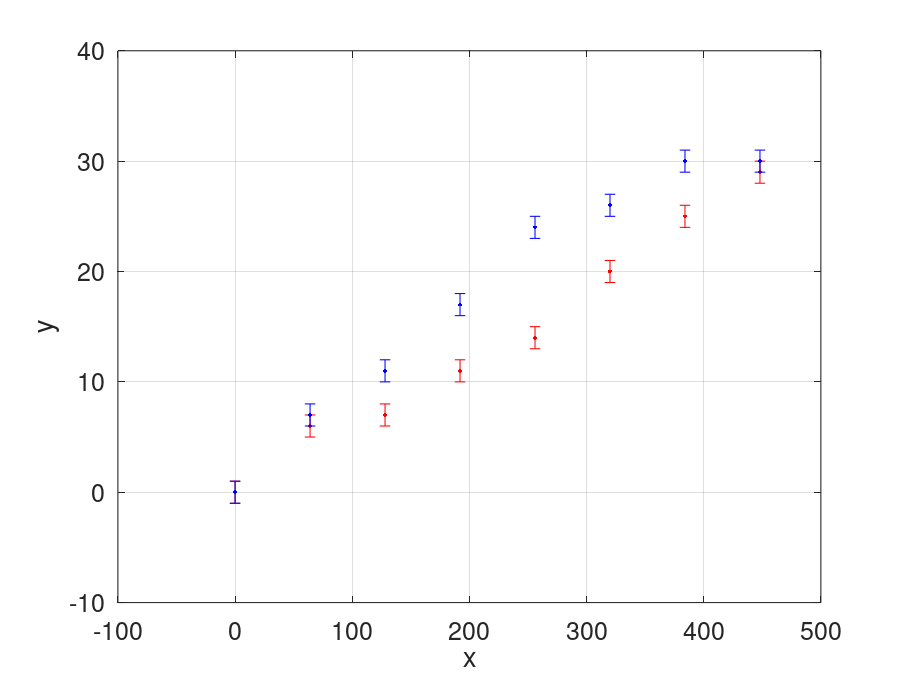
\includegraphics[width=14cm]{img/input.png}
            \caption{Исходные данные}
            \label{fig:info}
        \end{figure}
        
        Как было сказано в постановке, рассмотрим случай, когда погрешность измерений находится во входных данных. Используя (\ref{eq:x_interval}) и (\ref{eq:y_interval}) построим брусы совместности данных
        
        Получим 
        \begin{align*}
            y^{\text{block}} &= \{  [-1, 1],  [5, 8],   [6, 12],   [10, 18],   [13, 25],   [19, 27],   [24, 31],     [28, 31]\} \\
            x^{\text{block}} &= \{  [-13, 13],  [75, 120],   [90, 180],   [150, 270],   [194, 375],   [283, 402],   [360, 463],     [420, 463]\}
        \end{align*}
        
        \begin{figure}[H]
            \centering
            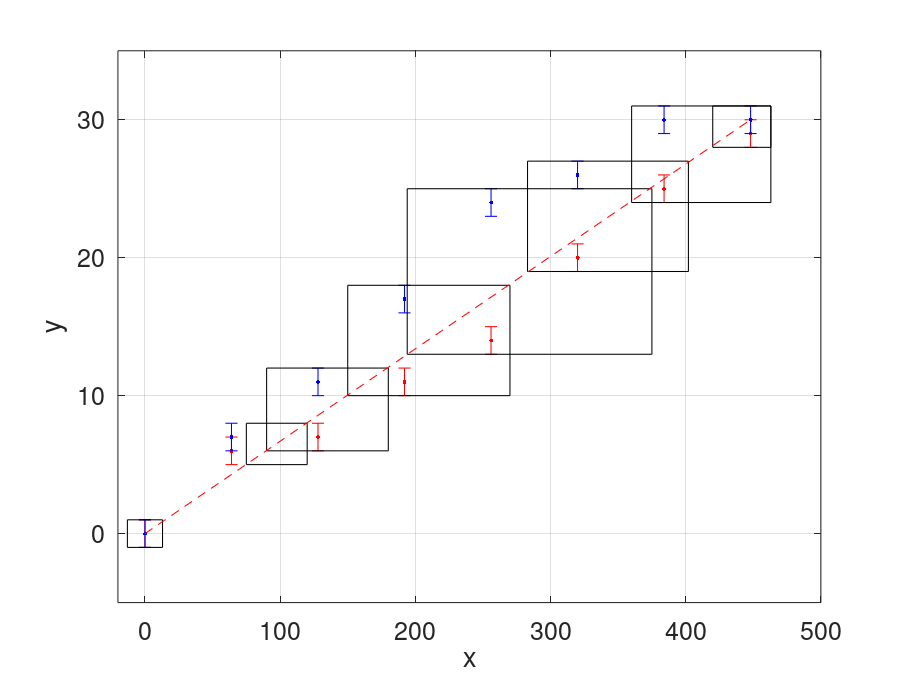
\includegraphics[width=14cm]{img/boxes.png}
            \caption{Брусы совместности данных}
            \label{fig:info}
        \end{figure}
        
        Составим вектор минимумов по включению для двух ветвей, который будем импользовать как набор данных для построения интервальной регрессии, используя следующее выражение
        
        \begin{equation}
            y_k = [\text{max}\{\underline{y}_{i}^{1}, \underline{y}_{i}^{2}\}, \text{min}\{\overline{y}_{i}^{1}, \overline{y}_{i}^{2}\}]
        \end{equation}
        
        Можем поставить задачу нахождения максимума совместности 
        \begin{equation}\label{eq:problem}
            X \cdot \beta \subseteq y
        \end{equation}
        
        Система иммет вид
        \begin{equation}\label{main_system}
            \begin{cases}
              [1, 1]\beta_{1} + [-13, 13]\beta_{2} = [-1, 1] \\
              [1, 1]\beta_{1} + [75, 120]\beta_{2} = [6, 7] \\
              [1, 1]\beta_{1} + [90, 180]\beta_{2} = [10, 8] \\
              [1, 1]\beta_{1} + [150, 270]\beta_{2} = [16, 12] \\
              [1, 1]\beta_{1} + [194, 375]\beta_{2} = [23, 15] \\
              [1, 1]\beta_{1} + [283, 402]\beta_{2} = [25, 21] \\
              [1, 1]\beta_{1} + [360, 463]\beta_{2} = [29, 26] \\
              [1, 1]\beta_{1} + [420, 463]\beta_{2} = [29, 30] 
            \end{cases}
        \end{equation}
        
        Данная система переопределенна. Решение - разбить исходную систему уравнений на квадратные подсистемы
        $$
            X^{i} \cdot \beta \subseteq y^{i}
        $$
        которые можно решать и рассматривать отдельно друг от друга
        
        Для каждой такой подсистемы найдем интервальные оценки параметров. Итоговые интервальные оценки для исходной системы уравнений будут результатом пересечения оценок, полученных из решения квадратных подсистем уравнений
        
        Пусть решениями подсистем будут множества 
        $$
            \Xi^{(1)}, ... , \Xi^{(k)}
        $$
        
        Составим пересечение этих множеств, которое будет оценкой решения системы включений (\ref{eq:problem})
        $$
            \Xi = \wedge \: \Xi^{(i)}
        $$
        
        Систему (\ref{main_system}) разобьем на 4 системы $2\text{x}2$, включая в системы 1 и 8, 2 и 7, 3 и 6, 4 и 5 уравнения
        
        \begin{equation}
             \begin{cases}
               [1, 1]\beta_{1} + [-13, 13]\beta_{2} = [-1, 1]\\
               [1, 1]\beta_{1} + [420, 463]\beta_{2} = [29, 30]
             \end{cases}
        \end{equation}
        
        \begin{equation}
             \begin{cases}
               [1, 1]\beta_{1} + [75, 120]\beta_{2} = [6, 7]\\
               [1, 1]\beta_{1} + [360, 463]\beta_{2} = [29, 26]
             \end{cases}
        \end{equation}
        
        \begin{equation}
             \begin{cases}
               [1, 1]\beta_{1} + [90, 180]\beta_{2} = [10, 8]\\
               [1, 1]\beta_{1} + [283, 402]\beta_{2} = [25, 21]
             \end{cases}
        \end{equation}
        
        \begin{equation}
             \begin{cases}
               [1, 1]\beta_{1} + [150, 270]\beta_{2} = [16, 12]\\
               [1, 1]\beta_{1} + [194, 375]\beta_{2} = [23, 15]
             \end{cases}
        \end{equation}
        
        Для каждой такой подсистемы запишем полученные результаты параметров
        \begin{align}
            \beta_{1}^{1} = [-0.16, 0.16]\\
               \beta_{2}^{1} = [0.07, 0.06]
        \end{align}
        \begin{align}
            \beta_{1}^{2} = [-7.86, 4.28]\\
               \beta_{2}^{2} = [0.16, 0.03]
        \end{align}
        \begin{align}
            \beta_{1}^{3} = [3, -2.54]\\
               \beta_{2}^{3} = [0.08, 0.06]
        \end{align}
        \begin{align}
            \beta_{1}^{4} = [-0.05, 0.35]\\
            \beta_{2}^{4} = [0.08, 0.05]
        \end{align}
        
        Пересечением значений $\beta_{1}^{i}$ и $\beta_{2}^{i}$ для подсистем получим значения параметров регрессии для исходной системы
        
        \begin{align*}
            \beta_{1} = \wedge \beta_{1}^{i} = [3, -2.54]\\
            \beta_{2} = \wedge \beta_{2}^{i} = [0.16, 0.03]
        \end{align*}
        
        Изобразим графически полученные результаты (зеленым цветом)
        
        \begin{figure}[H]
            \centering
            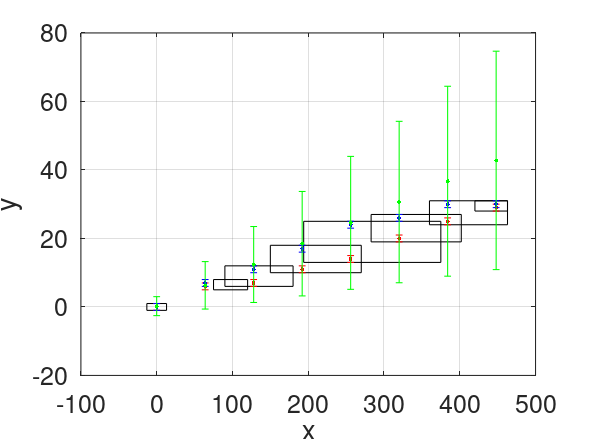
\includegraphics[width=14cm]{img/scores.png}
            \caption{Результаты}
            \label{fig:info}
        \end{figure}
        
        
    \section{Обсуждение}
        Пользуясь методом разбиения системы на квадратные подсистемы, нужно учитывать, что результаты очень сильно зависят от способа выбора квадратных подсистем. Так для рассмотренного разбиения для всех замеров полученные границы интервальных оценок выходят за пределы исходной диаграммы рассеивания
        
    \section{Приложения}
	    Код программы на GitHub, URL: \url{https://github.com/ViktorOneLove/computing_complexes}
        
\end{document}
